\subsection{Experimentación Final}

Para concluir este trabajo, tomamos el algoritmo de backtracking, el algoritmo goloso, el de busqueda local 1 y GRASP 1 y mediremos las diferencias de performance y de tiempos en cada uno para intentar sacar conclusiones.

Comenzaremos con un pequeño experimento variando $n$. Tomaremos grafos completos con $k = 5$, pesos aleaotrios en las aristas y variando la cantidad de nodos desde $1$ a $19$ y mediremos cuales son los k-PMP encontrados por cada algoritmo.

Los resultados arrojados por la experimentación pueden verse en el siguiente grafico:

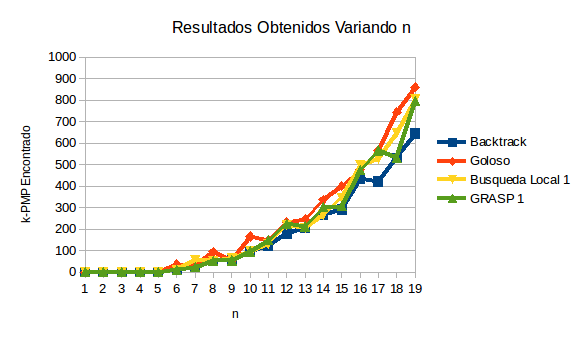
\includegraphics[scale=0.5]{Con/performance1.png}

Lo primero que podemos observar es que para casos triviales con $n$ <= $k$ todos son capaces de encontrar la respuesta optima.

Lo segundo que podemos observar, es que salvo un caso, el algoritmo goloso siempre pareciera ser el que encuentra las peores soluciones, llegando a obtener una respuesta un $33 \%$ alejada de la optima en el caso de $19$ nodos. (k-PMP encontrado por el backtrack: 644, k-PMP encontrado por la heuristica golosa: 860).

Las respuestas obtenidas por la busqueda local y el GRASP, resultan en general, en mucho mejores k-PMPs, desviandose hasta un $10\%$ de la respuesta por backtracking.

Ademas de estos 19 casos, podemos ver que el algoritmo goloso encuentra $6$ soluciones exactas (las 5 triviales y una para $n = 9$), la busqueda local encuentra $10$ respuestas exactas y el GRASP encuentra $11$ respuestas exactas. Si bien este el set de datos no es muy significativo, ya es posible ver las ventajas que representan las dos ultimas heuristicas frente a la primera.

Ademas, para estos 19 casos, medimos los tiempos que tardan en obtener una respuesta:

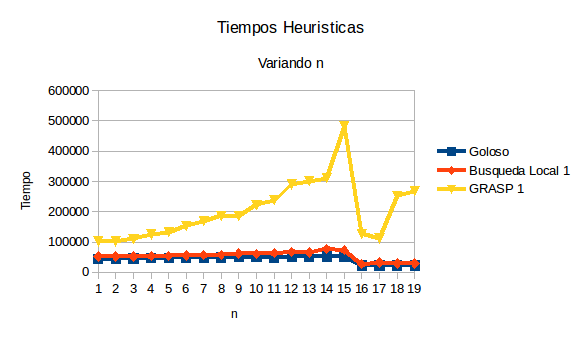
\includegraphics[scale=0.5]{Con/tiempos1Back.png}

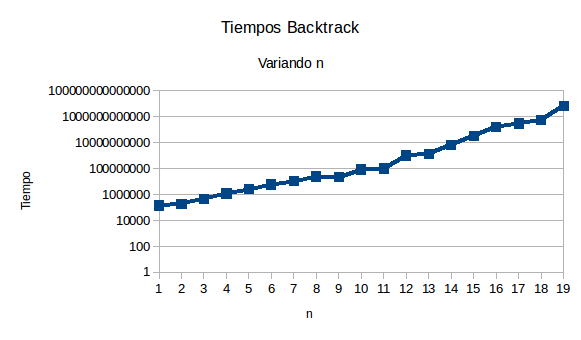
\includegraphics[scale=0.5]{Con/tiempos1Otros.png}

Como era de esperar, mietras que las heuristicas escalan de manera mas o menos polinomial, el backtracking escala de manera exponencial ascendiendo un orden de magnitud cada vez que asciende en uno el valor de $n$, hasta el punto que pasados los $19$ nodos, los tiempos empiezan a ser inviables.

\subsection{Experimentación Final}

En esta sección analizaremos cuantas respuestas exactas puede dar cada algoritmo para un grafo elegido mas o menos al azar. Para eso correremos el Backtrack sobre $100$ grafos de $19$ nodos completos, con pesos en las aristas aleaotrios entre 1 y 100 y $k = 4$ y veremos en cuantos casos cada algoritmo encuentra la respuesta exacta.

Las respuestas obtenidas son las siguientes:


\section{Conclusión}

Concluimos que dado un problema como $k-PMP$ el cual no conocemos algoritmos polinomiales para resolverlo de forma exacta, podemos utilizar las distintas técnicas algorítmicas para dar una solución en un tiempo razonable con la contrapartida de relajar los requerimientos de la misma. 

Vimos que la técnica de Metaheurística GRASP es una combinación válida entre distintos esquemas de algoritmos y trata de combinarlas para explorar el espacio de soluciones de una manera eficiente. En nuestro caso particular vimos que la implementación de GRASP 2 es la que mejores soluciones encontró. 

Como trabajo adicional habria que hacer pruebas más extensas en distintas familias de grafos conocidas para ver si nuestro algoritmo tiene casos patológicos aun no descubiertos los cuales su solución es tan mala como uno quisiera.